% Options for packages loaded elsewhere
\PassOptionsToPackage{unicode}{hyperref}
\PassOptionsToPackage{hyphens}{url}
\PassOptionsToPackage{dvipsnames,svgnames,x11names}{xcolor}
%
\documentclass[
  13pt,
  a4paper,
  DIV=11,
  numbers=noendperiod]{scrreprt}

\usepackage{amsmath,amssymb}
\usepackage{iftex}
\ifPDFTeX
  \usepackage[T1]{fontenc}
  \usepackage[utf8]{inputenc}
  \usepackage{textcomp} % provide euro and other symbols
\else % if luatex or xetex
  \usepackage{unicode-math}
  \defaultfontfeatures{Scale=MatchLowercase}
  \defaultfontfeatures[\rmfamily]{Ligatures=TeX,Scale=1}
\fi
\usepackage{lmodern}
\ifPDFTeX\else  
    % xetex/luatex font selection
\fi
% Use upquote if available, for straight quotes in verbatim environments
\IfFileExists{upquote.sty}{\usepackage{upquote}}{}
\IfFileExists{microtype.sty}{% use microtype if available
  \usepackage[]{microtype}
  \UseMicrotypeSet[protrusion]{basicmath} % disable protrusion for tt fonts
}{}
\makeatletter
\@ifundefined{KOMAClassName}{% if non-KOMA class
  \IfFileExists{parskip.sty}{%
    \usepackage{parskip}
  }{% else
    \setlength{\parindent}{0pt}
    \setlength{\parskip}{6pt plus 2pt minus 1pt}}
}{% if KOMA class
  \KOMAoptions{parskip=half}}
\makeatother
\usepackage{xcolor}
\usepackage[top=20mm,left=20mm]{geometry}
\setlength{\emergencystretch}{3em} % prevent overfull lines
\setcounter{secnumdepth}{2}
% Make \paragraph and \subparagraph free-standing
\ifx\paragraph\undefined\else
  \let\oldparagraph\paragraph
  \renewcommand{\paragraph}[1]{\oldparagraph{#1}\mbox{}}
\fi
\ifx\subparagraph\undefined\else
  \let\oldsubparagraph\subparagraph
  \renewcommand{\subparagraph}[1]{\oldsubparagraph{#1}\mbox{}}
\fi

\usepackage{color}
\usepackage{fancyvrb}
\newcommand{\VerbBar}{|}
\newcommand{\VERB}{\Verb[commandchars=\\\{\}]}
\DefineVerbatimEnvironment{Highlighting}{Verbatim}{commandchars=\\\{\}}
% Add ',fontsize=\small' for more characters per line
\usepackage{framed}
\definecolor{shadecolor}{RGB}{241,243,245}
\newenvironment{Shaded}{\begin{snugshade}}{\end{snugshade}}
\newcommand{\AlertTok}[1]{\textcolor[rgb]{0.68,0.00,0.00}{#1}}
\newcommand{\AnnotationTok}[1]{\textcolor[rgb]{0.37,0.37,0.37}{#1}}
\newcommand{\AttributeTok}[1]{\textcolor[rgb]{0.40,0.45,0.13}{#1}}
\newcommand{\BaseNTok}[1]{\textcolor[rgb]{0.68,0.00,0.00}{#1}}
\newcommand{\BuiltInTok}[1]{\textcolor[rgb]{0.00,0.23,0.31}{#1}}
\newcommand{\CharTok}[1]{\textcolor[rgb]{0.13,0.47,0.30}{#1}}
\newcommand{\CommentTok}[1]{\textcolor[rgb]{0.37,0.37,0.37}{#1}}
\newcommand{\CommentVarTok}[1]{\textcolor[rgb]{0.37,0.37,0.37}{\textit{#1}}}
\newcommand{\ConstantTok}[1]{\textcolor[rgb]{0.56,0.35,0.01}{#1}}
\newcommand{\ControlFlowTok}[1]{\textcolor[rgb]{0.00,0.23,0.31}{#1}}
\newcommand{\DataTypeTok}[1]{\textcolor[rgb]{0.68,0.00,0.00}{#1}}
\newcommand{\DecValTok}[1]{\textcolor[rgb]{0.68,0.00,0.00}{#1}}
\newcommand{\DocumentationTok}[1]{\textcolor[rgb]{0.37,0.37,0.37}{\textit{#1}}}
\newcommand{\ErrorTok}[1]{\textcolor[rgb]{0.68,0.00,0.00}{#1}}
\newcommand{\ExtensionTok}[1]{\textcolor[rgb]{0.00,0.23,0.31}{#1}}
\newcommand{\FloatTok}[1]{\textcolor[rgb]{0.68,0.00,0.00}{#1}}
\newcommand{\FunctionTok}[1]{\textcolor[rgb]{0.28,0.35,0.67}{#1}}
\newcommand{\ImportTok}[1]{\textcolor[rgb]{0.00,0.46,0.62}{#1}}
\newcommand{\InformationTok}[1]{\textcolor[rgb]{0.37,0.37,0.37}{#1}}
\newcommand{\KeywordTok}[1]{\textcolor[rgb]{0.00,0.23,0.31}{#1}}
\newcommand{\NormalTok}[1]{\textcolor[rgb]{0.00,0.23,0.31}{#1}}
\newcommand{\OperatorTok}[1]{\textcolor[rgb]{0.37,0.37,0.37}{#1}}
\newcommand{\OtherTok}[1]{\textcolor[rgb]{0.00,0.23,0.31}{#1}}
\newcommand{\PreprocessorTok}[1]{\textcolor[rgb]{0.68,0.00,0.00}{#1}}
\newcommand{\RegionMarkerTok}[1]{\textcolor[rgb]{0.00,0.23,0.31}{#1}}
\newcommand{\SpecialCharTok}[1]{\textcolor[rgb]{0.37,0.37,0.37}{#1}}
\newcommand{\SpecialStringTok}[1]{\textcolor[rgb]{0.13,0.47,0.30}{#1}}
\newcommand{\StringTok}[1]{\textcolor[rgb]{0.13,0.47,0.30}{#1}}
\newcommand{\VariableTok}[1]{\textcolor[rgb]{0.07,0.07,0.07}{#1}}
\newcommand{\VerbatimStringTok}[1]{\textcolor[rgb]{0.13,0.47,0.30}{#1}}
\newcommand{\WarningTok}[1]{\textcolor[rgb]{0.37,0.37,0.37}{\textit{#1}}}

\providecommand{\tightlist}{%
  \setlength{\itemsep}{0pt}\setlength{\parskip}{0pt}}\usepackage{longtable,booktabs,array}
\usepackage{calc} % for calculating minipage widths
% Correct order of tables after \paragraph or \subparagraph
\usepackage{etoolbox}
\makeatletter
\patchcmd\longtable{\par}{\if@noskipsec\mbox{}\fi\par}{}{}
\makeatother
% Allow footnotes in longtable head/foot
\IfFileExists{footnotehyper.sty}{\usepackage{footnotehyper}}{\usepackage{footnote}}
\makesavenoteenv{longtable}
\usepackage{graphicx}
\makeatletter
\def\maxwidth{\ifdim\Gin@nat@width>\linewidth\linewidth\else\Gin@nat@width\fi}
\def\maxheight{\ifdim\Gin@nat@height>\textheight\textheight\else\Gin@nat@height\fi}
\makeatother
% Scale images if necessary, so that they will not overflow the page
% margins by default, and it is still possible to overwrite the defaults
% using explicit options in \includegraphics[width, height, ...]{}
\setkeys{Gin}{width=\maxwidth,height=\maxheight,keepaspectratio}
% Set default figure placement to htbp
\makeatletter
\def\fps@figure{htbp}
\makeatother
% definitions for citeproc citations
\NewDocumentCommand\citeproctext{}{}
\NewDocumentCommand\citeproc{mm}{%
  \begingroup\def\citeproctext{#2}\cite{#1}\endgroup}
\makeatletter
 % allow citations to break across lines
 \let\@cite@ofmt\@firstofone
 % avoid brackets around text for \cite:
 \def\@biblabel#1{}
 \def\@cite#1#2{{#1\if@tempswa , #2\fi}}
\makeatother
\newlength{\cslhangindent}
\setlength{\cslhangindent}{1.5em}
\newlength{\csllabelwidth}
\setlength{\csllabelwidth}{3em}
\newenvironment{CSLReferences}[2] % #1 hanging-indent, #2 entry-spacing
 {\begin{list}{}{%
  \setlength{\itemindent}{0pt}
  \setlength{\leftmargin}{0pt}
  \setlength{\parsep}{0pt}
  % turn on hanging indent if param 1 is 1
  \ifodd #1
   \setlength{\leftmargin}{\cslhangindent}
   \setlength{\itemindent}{-1\cslhangindent}
  \fi
  % set entry spacing
  \setlength{\itemsep}{#2\baselineskip}}}
 {\end{list}}
\usepackage{calc}
\newcommand{\CSLBlock}[1]{\hfill\break\parbox[t]{\linewidth}{\strut\ignorespaces#1\strut}}
\newcommand{\CSLLeftMargin}[1]{\parbox[t]{\csllabelwidth}{\strut#1\strut}}
\newcommand{\CSLRightInline}[1]{\parbox[t]{\linewidth - \csllabelwidth}{\strut#1\strut}}
\newcommand{\CSLIndent}[1]{\hspace{\cslhangindent}#1}

%mine
\usepackage{amsmath}
\usepackage{braket}
\addtokomafont{disposition}{\rmfamily}
\usepackage{fvextra}
\DefineVerbatimEnvironment{Highlighting}{Verbatim}{breaklines,commandchars=\\\{\}}
\KOMAoption{captions}{tableheading}
\makeatletter
\@ifpackageloaded{bookmark}{}{\usepackage{bookmark}}
\makeatother
\makeatletter
\@ifpackageloaded{caption}{}{\usepackage{caption}}
\AtBeginDocument{%
\ifdefined\contentsname
  \renewcommand*\contentsname{Table of contents}
\else
  \newcommand\contentsname{Table of contents}
\fi
\ifdefined\listfigurename
  \renewcommand*\listfigurename{List of Figures}
\else
  \newcommand\listfigurename{List of Figures}
\fi
\ifdefined\listtablename
  \renewcommand*\listtablename{List of Tables}
\else
  \newcommand\listtablename{List of Tables}
\fi
\ifdefined\figurename
  \renewcommand*\figurename{Figure}
\else
  \newcommand\figurename{Figure}
\fi
\ifdefined\tablename
  \renewcommand*\tablename{Table}
\else
  \newcommand\tablename{Table}
\fi
}
\@ifpackageloaded{float}{}{\usepackage{float}}
\floatstyle{ruled}
\@ifundefined{c@chapter}{\newfloat{codelisting}{h}{lop}}{\newfloat{codelisting}{h}{lop}[chapter]}
\floatname{codelisting}{Listing}
\newcommand*\listoflistings{\listof{codelisting}{List of Listings}}
\makeatother
\makeatletter
\makeatother
\makeatletter
\@ifpackageloaded{caption}{}{\usepackage{caption}}
\@ifpackageloaded{subcaption}{}{\usepackage{subcaption}}
\makeatother
\ifLuaTeX
\usepackage[bidi=basic]{babel}
\else
\usepackage[bidi=default]{babel}
\fi
\babelprovide[main,import]{english}
% get rid of language-specific shorthands (see #6817):
\let\LanguageShortHands\languageshorthands
\def\languageshorthands#1{}
\ifLuaTeX
  \usepackage{selnolig}  % disable illegal ligatures
\fi
\usepackage{bookmark}

\IfFileExists{xurl.sty}{\usepackage{xurl}}{} % add URL line breaks if available
\urlstyle{same} % disable monospaced font for URLs
\hypersetup{
  pdftitle={Hierarchical quantum circuit representation for music genre classification},
  pdfauthor={Ludovico Venturi},
  pdflang={en},
  colorlinks=true,
  linkcolor={blue},
  filecolor={Maroon},
  citecolor={Blue},
  urlcolor={Blue},
  pdfcreator={LaTeX via pandoc}}

\title{Hierarchical quantum circuit representation for music genre
classification}
\author{Ludovico Venturi}
\date{}

\begin{document}
\maketitle

\RecustomVerbatimEnvironment{verbatim}{Verbatim}{
  showspaces = false,
  showtabs = false,
  breaksymbolleft={},
  breaklines
  % Note: setting commandchars=\\\{\} here will cause an error 
}

\renewcommand*\contentsname{Table of contents}
{
\hypersetup{linkcolor=}
\setcounter{tocdepth}{2}
\tableofcontents
}
\bookmarksetup{startatroot}

\chapter*{Abstract}\label{abstract}
\addcontentsline{toc}{chapter}{Abstract}

\markboth{Abstract}{Abstract}

In this project work I tried to replicate some of the results of the
paper ``Hierarchical quantum circuit representations for neural
architecture search'' {[}\citeproc{ref-lourens2023hierarchical}{1}{]}.

In this paper the authors propose a framework named HierarQcal for
representing Quantum Convolutional Neural Networks (QCNN) architectures
using techniques from Neural Architectural Search (NAS). This framework
enables search space design and architecture search, the former being
the most challenging point in applying NAS to QCNN.

In this work I generate the family of QCNN architectures resembling
reverse binary trees and I evaluate this family on the GTZAN music genre
classification dataset showing that it is possible to improve model
performance without increasing complexity.

\bookmarksetup{startatroot}

\chapter{Background}\label{background}

\section{Supervised Learning for
classification}\label{supervised-learning-for-classification}

The goal of classification is to use some data \(X\) alongside a
function \(f_m\) (model) to accurately represent a discrete
categorization \(y\): \[
f_m(X, \theta) = \widehat{y} \approx y
\]

The data is used by iteratively changing the model parameters \(\theta\)
based on the disparity between the current representation
\(\widehat{y}\) and the actual categorization \(y\), measured with a
cost function \(C(y, \widehat{y})\). It's a supervised problem because
the label of each input is known from the start.

The cost function I use in this project is Binary Cross Entropy (BCE)
from \texttt{torch.nn.BCELoss}. Cross-entropy is a measure of the
difference between two probability distributions for a given random
variable or set of events. In other words, if we consider a target
probability distribution \(P\) and an approximation of the target
distribution \(Q\), then the cross-entropy of \(Q\) from \(P\) is the
number of additional bits to represent an event using \(Q\) instead of
\(P\): \[
H(P,Q) = - \sum_{x \in X} P(x) \cdot ln(Q(x))
\]

\section{Convolutional Neural
Networks}\label{convolutional-neural-networks}

Convolutional Neural Networks (CNN) are successful because they don't
need manual feature design and can learn high-level features from raw
data. With CNN there is a focus shift: from feature design to
architecture design.

\ldots.

\section{Quantum Machine Learning}\label{quantum-machine-learning}

Using quantum computers it is possible to write hybrid quantum-classical
algorithms already usable in the NISQ era, where the optimization of
parameters is done classically and the function \(f_m\) is built as a
Variational Quantum Circuit (VQC) that acts on a quantum state
\(\ket{\psi}\).

A VQC is a quantum circuit with trainable parameters in some gates, as a
rotation angle \(\theta, e.g. RY(\theta)\).

The point in using a VQC is that the state can move along all Hilbert
space at every change of the parameters, so it is possible to sample
from a classically intractable probability density function (pdf).

\begin{figure}

\centering{

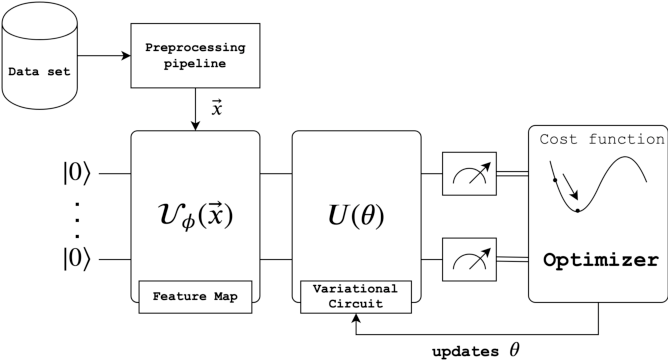
\includegraphics{chapters/../img/vqc.png}

}

\caption{\label{fig-vqc}Variational Quantum Circuit
{[}\citeproc{ref-vqc_tut}{2}{]}}

\end{figure}%

\subsection{Data encoding}\label{data-encoding}

The state \(\ket{\psi}\) must be obtained through an embedding since
we're in a Classical-Quantum (CQ) setting and the data we use for
training is classic. This is done with a \emph{feature map}, as can be
seen in Figure~\ref{fig-vqc}.

A quantum embedding represents classical data as quantum states in a
Hilbert space via a quantum feature map. It takes a classical data \(x\)
and translates it into a set of gate parameters in a quantum circuit,
creating a quantum state \(\ket{\psi_x}\).

In this project I use \emph{angle embedding} to encode classical data
(audio statistics) to the circuit (see line 10 in
Figure~\ref{fig-code_circuit}). With angle embedding, single-qubit
rotation gates encode a classical \(x_i \in \mathcal{R}\).

Each element of the input determines the angle of the rotation gate
(e.g.~an RY rotation gate). This approach requires \(n\) qubits to
encode \(n\) input variables and can be defined as: \[
\ket{\psi_x} = \bigotimes_{i=1}^n cos(x_i) \ket{0} + sin(x_i)\ket{1} = \bigotimes_{i=1}^n R(x_i)\ket{\psi_0}
\]

\subsection{QCNNs}\label{qcnns}

QCNN stands out among other parametrized quantum circuits (PQC) models
for its shallow circuit depth, good generalization capabilities and
absence of \emph{barren plateaus}.

A \emph{barren plateau} happens when the gradient of a cost function
vanishes exponentially with system size, rendering the architecture
untrainable for large problem sizes. For PQC, random circuits are often
proposed as initial guesses for exploring the space of quantum states,
due to exponential dimension of Hilbert space and the gradient
estimation complexity on more than a few qubits.

It is important to note that for a wide class of PQC the probability
that the gradient along any reasonable direction is non-zero to some
fixed precision is exponentially small as a function of the number of
qubits {[}\citeproc{ref-McClean2018Nov}{3}{]}. For QCNN in particular it
is guaranteed that randomly initialized QCNN are trainable unlike many
other PQC architectures, since the variance of the gradient vanishes no
faster than polynomially {[}\citeproc{ref-Pesah2021Oct}{4}{]} so QCNNs
do not exhibit \emph{barren plateaus}.

The next step is learning network architecture, which NAS aims to
achieve {[}\citeproc{ref-elsken2019neural}{5}{]}. NAS consists of 3 main
components:

\begin{itemize}
\tightlist
\item
  search space
\item
  search strategy
\item
  performance estimation strategy
\end{itemize}

The \emph{search space} defines the set of possible architectures that a
search algorithm can consider, and a carefully designed search space is
important for search efficiency. The main contribution of
{[}\citeproc{ref-lourens2023hierarchical}{1}{]} is a framework that
enables the dynamic generation of QCNN and the creation of QCNN search
spaces: HierarQcal.

\section{HierarQcal}\label{hierarqcal}

HierarQcal is an open-source python package
{[}\citeproc{ref-github_hierarqcal}{6}{]} that simplifies the process of
creating general QCNN by enabling an hierarchical design process. It
makes automatic generation of QCNN circuits easy and it facilitates QCNN
search space design for NAS.

The package includes primitives such as \emph{convolutions, pooling} and
\emph{dense layers} that can be stacked together hierarchically to form
complex QCNN circuit architectures.

\ldots.

\bookmarksetup{startatroot}

\chapter{Methods}\label{methods}

\section{Dataset}\label{dataset}

The GTZAN dataset
{[}\citeproc{ref-gtzan_tzanetakis_essl_cook_2001}{7}{]} is the most-used
public dataset for evaluation in machine listening research for music
genre recognition (MGR). The files were collected in 2000-2001 from a
variety of sources including personal CDs, radio, microphone recordings,
in order to represent a variety of recording conditions.

The dataset consists of 1000 audio tracks each 30 seconds long. It
contains 10 genres, each represented by 100 tracks. The tracks are all
22050Hz Mono 16-bit audio files in \texttt{.wav} format. The genres are:
blues,classical, country, disco, hiphop, jazz, metal, pop, reggae, rock.

I used the GTZAN dataset from Kaggle
{[}\citeproc{ref-GTZAN_kaggle}{8}{]}, which already include statistics
extracted from the audio sources. The information gathered from audio
signals to produce the tabular dataset can be easily extracted with
\texttt{librosa} \footnote{a Python package for audio and music signal
  processing {[}\citeproc{ref-mcfee2015librosa}{9}{]}} and contains:
Chroma frequencies, Harmonic and percussive elements, Mel-frequency
cepstral coefficients, Spectral bandwidth and others. For a description
of these and other features see Appendix D of
{[}\citeproc{ref-lourens2023hierarchical}{1}{]}.

I did binary classification in this analysis, in particular I focused
only on \emph{rock vs country} classification, the most difficult task
between all the \(\binom{10}{2} = 45\) possible genre pairs.

\section{Model implementation}\label{model-implementation}

\subsection{Main workflow}\label{main-workflow}

Data is first preprocessed in two ways:

\begin{itemize}
\tightlist
\item
  feature scaling\\
\item
  feature reduction
\end{itemize}

Features are scaled using \texttt{min-max} scaling in a range chosen for
angle embedding: \([0, \pi/2]\). Then Principal Component Anaylisis with
8 components is used to perform the reduction.

I used \texttt{sklearn} for both operations. I also used
\texttt{Pipeline} from \texttt{sklearn} to create a preprocessing
pipeline that will be used for the search of hyperparameters (that will
be discussed in Section~\ref{sec-hyp_search}).

\begin{Shaded}
\begin{Highlighting}[numbers=left,,]
\ImportTok{from}\NormalTok{ sklearn.preprocessing }\ImportTok{import}\NormalTok{ MinMaxScaler}
\ImportTok{from}\NormalTok{ sklearn.decomposition }\ImportTok{import}\NormalTok{ PCA}
\ImportTok{from}\NormalTok{ sklearn.pipeline }\ImportTok{import}\NormalTok{ Pipeline}

\NormalTok{pipeline }\OperatorTok{=}\NormalTok{ Pipeline(}
\NormalTok{    [}
\NormalTok{        (}\StringTok{"scaler"}\NormalTok{, MinMaxScaler((}\DecValTok{0}\NormalTok{, np.pi }\OperatorTok{/} \DecValTok{2}\NormalTok{))),}
\NormalTok{        (}\StringTok{"pca"}\NormalTok{, PCA(}\DecValTok{8}\NormalTok{)),}
\NormalTok{    ]}
\NormalTok{)}
\end{Highlighting}
\end{Shaded}

Each row of the data resulting from the preprocessing has 8 features and
so it can be encoded through an angle embedding into a quantum circuit
with 8 qubit. The quantum circuit used here is a QCNN with a
hierarchical design: the idea is to reduce the system size in half until
one qubit remains while alternating between convolution and pooling
operations. Grant et al. {[}\citeproc{ref-grant2018hierarchical}{10}{]}
exhibited the success of hierarchical designs that resemble reverse
binary trees. To create a space of these architectures only three levels
of motifs are needed.

\begin{figure}[H]

{\centering 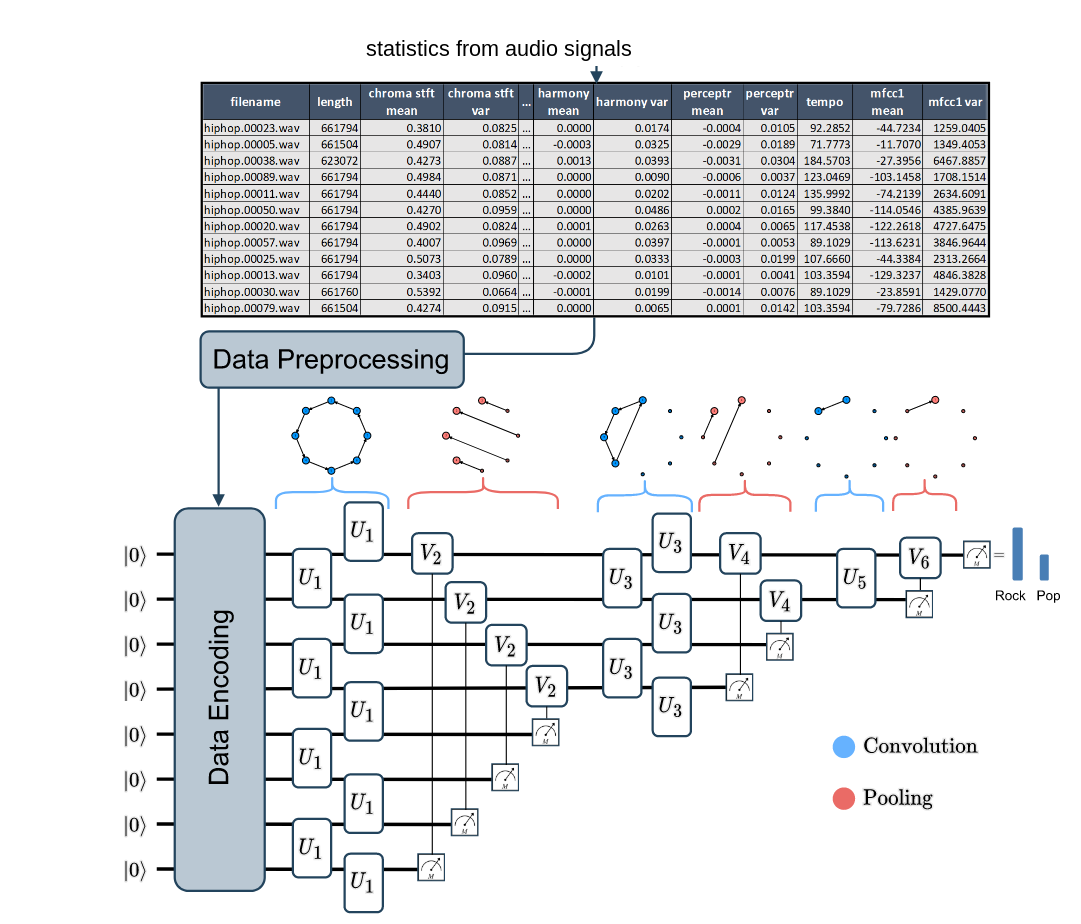
\includegraphics{chapters/../img/workflow.png}

}

\caption{Main workflow of model implementation. \(U\)s are convolutional
unitaries and \(V\)s a re pooling unitaries. From
{[}\citeproc{ref-lourens2023hierarchical}{1}{]}}

\end{figure}%

I used \(N = 8\) qubits with pennylane \texttt{default.qubit.torch} as
simulation device (see line 2 in Figure~\ref{fig-code_circuit}). I
tested each model based on different combinations of model architecture
(that will be discussed in more detail later) and two-qubit unitary
ansatzes.

\subsection{Ansatzes}\label{ansatzes}

I used 3 out of the 8 proposed ansatzes in Lourens et al.
{[}\citeproc{ref-lourens2023hierarchical}{1}{]}, in particular:

\begin{figure}

\centering{

\captionsetup{labelsep=none}

\begin{figure}[H]

{\centering 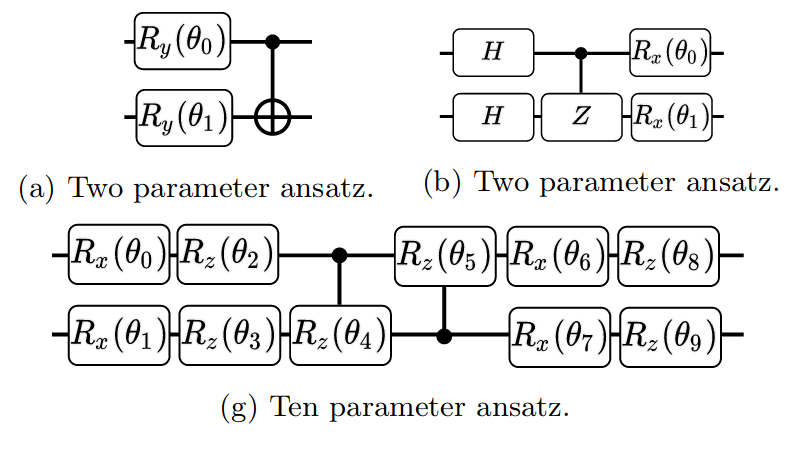
\includegraphics{chapters/../img/ansatzes_conv.png}

}

\caption{Convolution ansatzes used in this project, from
{[}\citeproc{ref-lourens2023hierarchical}{1}{]}}

\end{figure}%

}

\caption{\label{fig-conv_ansatzes}}

\end{figure}%

Below there is the correspondent code for each ansatz:

\begin{Shaded}
\begin{Highlighting}[]
\CommentTok{\# Convolution ansatz (a) }
\KeywordTok{def}\NormalTok{ ansatz\_conv\_a(bits, symbols}\OperatorTok{=}\VariableTok{None}\NormalTok{):}
\NormalTok{  qml.RY(symbols[}\DecValTok{0}\NormalTok{], wires}\OperatorTok{=}\NormalTok{[bits[}\DecValTok{0}\NormalTok{]])}
\NormalTok{  qml.RY(symbols[}\DecValTok{1}\NormalTok{], wires}\OperatorTok{=}\NormalTok{[bits[}\DecValTok{1}\NormalTok{]])}
\NormalTok{  qml.CNOT(wires}\OperatorTok{=}\NormalTok{[bits[}\DecValTok{0}\NormalTok{], bits[}\DecValTok{1}\NormalTok{]])}
\NormalTok{U\_ansatz\_conv\_a }\OperatorTok{=}\NormalTok{ Qunitary(ansatz\_conv\_a, n\_symbols}\OperatorTok{=}\DecValTok{2}\NormalTok{, arity}\OperatorTok{=}\DecValTok{2}\NormalTok{)}

\CommentTok{\# Convolution ansatz (b) }
\KeywordTok{def}\NormalTok{ ansatz\_conv\_b(bits, symbols}\OperatorTok{=}\VariableTok{None}\NormalTok{):}
\NormalTok{  qml.Hadamard(wires}\OperatorTok{=}\NormalTok{[bits[}\DecValTok{0}\NormalTok{]])}
\NormalTok{  qml.Hadamard(wires}\OperatorTok{=}\NormalTok{[bits[}\DecValTok{1}\NormalTok{]])}
\NormalTok{  qml.CZ(wires}\OperatorTok{=}\NormalTok{[bits[}\DecValTok{0}\NormalTok{], bits[}\DecValTok{1}\NormalTok{]])}
\NormalTok{  qml.RX(symbols[}\DecValTok{0}\NormalTok{], wires}\OperatorTok{=}\NormalTok{[bits[}\DecValTok{0}\NormalTok{]])}
\NormalTok{  qml.RX(symbols[}\DecValTok{1}\NormalTok{], wires}\OperatorTok{=}\NormalTok{[bits[}\DecValTok{1}\NormalTok{]])}
\NormalTok{U\_ansatz\_conv\_b }\OperatorTok{=}\NormalTok{ Qunitary(ansatz\_conv\_b, n\_symbols}\OperatorTok{=}\DecValTok{2}\NormalTok{, arity}\OperatorTok{=}\DecValTok{2}\NormalTok{)}

\CommentTok{\# Convolution ansatz (g) }
\KeywordTok{def}\NormalTok{ ansatz\_conv\_g(bits, symbols):}
\NormalTok{    qml.RX(symbols[}\DecValTok{0}\NormalTok{], wires}\OperatorTok{=}\NormalTok{bits[}\DecValTok{0}\NormalTok{])}
\NormalTok{    qml.RX(symbols[}\DecValTok{1}\NormalTok{], wires}\OperatorTok{=}\NormalTok{bits[}\DecValTok{1}\NormalTok{])}
\NormalTok{    qml.RZ(symbols[}\DecValTok{2}\NormalTok{], wires}\OperatorTok{=}\NormalTok{bits[}\DecValTok{0}\NormalTok{])}
\NormalTok{    qml.RZ(symbols[}\DecValTok{3}\NormalTok{], wires}\OperatorTok{=}\NormalTok{bits[}\DecValTok{1}\NormalTok{])}
\NormalTok{    qml.CRZ(symbols[}\DecValTok{4}\NormalTok{], wires}\OperatorTok{=}\NormalTok{[bits[}\DecValTok{1}\NormalTok{], bits[}\DecValTok{0}\NormalTok{]])}
\NormalTok{    qml.CRZ(symbols[}\DecValTok{5}\NormalTok{], wires}\OperatorTok{=}\NormalTok{[bits[}\DecValTok{0}\NormalTok{], bits[}\DecValTok{1}\NormalTok{]])}
\NormalTok{    qml.RX(symbols[}\DecValTok{6}\NormalTok{], wires}\OperatorTok{=}\NormalTok{bits[}\DecValTok{0}\NormalTok{])}
\NormalTok{    qml.RX(symbols[}\DecValTok{7}\NormalTok{], wires}\OperatorTok{=}\NormalTok{bits[}\DecValTok{1}\NormalTok{])}
\NormalTok{    qml.RZ(symbols[}\DecValTok{8}\NormalTok{], wires}\OperatorTok{=}\NormalTok{bits[}\DecValTok{0}\NormalTok{])}
\NormalTok{    qml.RZ(symbols[}\DecValTok{9}\NormalTok{], wires}\OperatorTok{=}\NormalTok{bits[}\DecValTok{1}\NormalTok{])}
\NormalTok{U\_ansatz\_conv\_g }\OperatorTok{=}\NormalTok{ Qunitary(ansatz\_conv\_g, n\_symbols}\OperatorTok{=}\DecValTok{10}\NormalTok{, arity}\OperatorTok{=}\DecValTok{2}\NormalTok{)}
\end{Highlighting}
\end{Shaded}

For pooling ansatz I used:

\begin{figure}

\begin{minipage}{0.50\linewidth}

\begin{figure}[H]

{\centering 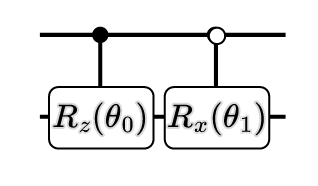
\includegraphics[width=\textwidth,height=1.5625in]{chapters/../img/ansatz_pool.png}

}

\subcaption{(1) Pooling ansatz from {[}\citeproc{ref-Hur2022Jun}{11}{]}}

\end{figure}%

\end{minipage}%
%
\begin{minipage}{0.50\linewidth}

\begin{figure}[H]

{\centering 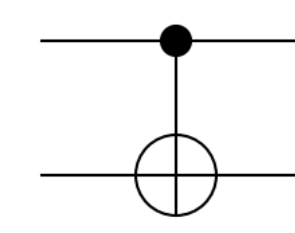
\includegraphics[width=\textwidth,height=1.45833in]{chapters/../img/ansatz_pool_simpler.png}

}

\subcaption{(2) Simpler pooling ansatz}

\end{figure}%

\end{minipage}%

\caption{\label{fig-pool-ansatz}Pooling ansatzes}

\end{figure}%

\subsection{Circuit}\label{circuit}

The code below illustrates how a general motif that resembles reverse
binary trees is built using HierarQcal. This motif is the base for every
model I used in this project.

\begin{Shaded}
\begin{Highlighting}[numbers=left,,]
\KeywordTok{def}\NormalTok{ qcnn\_motif(ansatz\_c, conv\_stride, conv\_step, conv\_offset, share\_weights, ansatz\_p, pool\_filter, pool\_stride):}
\NormalTok{    qcnn }\OperatorTok{=}\NormalTok{ (}
\NormalTok{        Qinit(}\DecValTok{8}\NormalTok{)}
        \OperatorTok{+}\NormalTok{ (}
\NormalTok{            Qcycle(}
\NormalTok{                stride}\OperatorTok{=}\NormalTok{conv\_stride,}
\NormalTok{                step}\OperatorTok{=}\NormalTok{conv\_step,}
\NormalTok{                offset}\OperatorTok{=}\NormalTok{conv\_offset,}
\NormalTok{                mapping}\OperatorTok{=}\NormalTok{ansatz\_c,}
\NormalTok{                share\_weights}\OperatorTok{=}\NormalTok{share\_weights,}
\NormalTok{            )}
            \OperatorTok{+}\NormalTok{ Qmask(pool\_filter, mapping}\OperatorTok{=}\NormalTok{ansatz\_p, strides}\OperatorTok{=}\NormalTok{pool\_stride)}
\NormalTok{        )}
        \OperatorTok{*} \DecValTok{3}
\NormalTok{    )}

    \ControlFlowTok{return}\NormalTok{ qcnn}
\end{Highlighting}
\end{Shaded}

The motif obtained from \texttt{qcnn\_motif} is not ready to be
executed. It needs to be translated to a pennylane circuit and also the
input \(x \in \mathcal{R}^8\) must be embedded into this circuit.

\begin{figure}

\centering{

\captionsetup{labelsep=none}

\begin{Shaded}
\begin{Highlighting}[numbers=left,,]
\KeywordTok{def}\NormalTok{ get\_circuit(hierq, x}\OperatorTok{=}\VariableTok{None}\NormalTok{):}
\NormalTok{    dev }\OperatorTok{=}\NormalTok{ qml.device(}\StringTok{"default.qubit.torch"}\NormalTok{, wires}\OperatorTok{=}\NormalTok{hierq.tail.Q, shots}\OperatorTok{=}\VariableTok{None}\NormalTok{)}

    \AttributeTok{@qml.qnode}\NormalTok{(dev, interface}\OperatorTok{=}\StringTok{"torch"}\NormalTok{, diff\_method}\OperatorTok{=}\StringTok{"backprop"}\NormalTok{)}
    \KeywordTok{def}\NormalTok{ circuit():}
        \ControlFlowTok{if} \BuiltInTok{isinstance}\NormalTok{(}\BuiltInTok{next}\NormalTok{(hierq.get\_symbols(), }\VariableTok{False}\NormalTok{), sp.Symbol):}
            \CommentTok{\# Pennylane doesn\textquotesingle{}t support symbolic parameters, so if no symbols were set (i.e. they are still symbolic), we initialize them randomly}
\NormalTok{            hierq.set\_symbols(np.random.uniform(}\DecValTok{0}\NormalTok{, }\DecValTok{2} \OperatorTok{*}\NormalTok{ np.pi, hierq.n\_symbols))}
        \ControlFlowTok{if}\NormalTok{ x }\KeywordTok{is} \KeywordTok{not} \VariableTok{None}\NormalTok{:}
\NormalTok{            AngleEmbedding(x, wires}\OperatorTok{=}\NormalTok{hierq.tail.Q, rotation}\OperatorTok{=}\StringTok{"Y"}\NormalTok{)}
\NormalTok{        hierq(backend}\OperatorTok{=}\StringTok{"pennylane"}\NormalTok{)  }\CommentTok{\# This executes the compute graph in order}
        \ControlFlowTok{return}\NormalTok{ qml.probs(wires}\OperatorTok{=}\NormalTok{hierq.head.Q[}\DecValTok{0}\NormalTok{])}

    \ControlFlowTok{return}\NormalTok{ circuit}
\end{Highlighting}
\end{Shaded}

}

\caption{\label{fig-code_circuit}}

\end{figure}%

The real execution with input \texttt{x} and circuit parameters
\texttt{symbols} is done with:

\begin{Shaded}
\begin{Highlighting}[numbers=left,,]
\KeywordTok{def}\NormalTok{ net(motif, symbols, x):}
\NormalTok{    motif.set\_symbols(symbols)}
\NormalTok{    circuit }\OperatorTok{=}\NormalTok{ get\_circuit(motif, x)}
\NormalTok{    y\_hat }\OperatorTok{=}\NormalTok{ circuit()}

    \ControlFlowTok{return}\NormalTok{ y\_hat}
\end{Highlighting}
\end{Shaded}

\subsection{Training}\label{training}

The dataset has been split in 70\% training set and 30\% test set.
During training, 3-fold cross validation is used for each model. This
step is automated during the search for hyperparameters.

\begin{figure}

\centering{

\captionsetup{labelsep=none}

\begin{Shaded}
\begin{Highlighting}[numbers=left,,]
\KeywordTok{def}\NormalTok{ train(x, y, motif, N}\OperatorTok{=}\DecValTok{100}\NormalTok{, lr}\OperatorTok{=}\FloatTok{0.1}\NormalTok{, verbose}\OperatorTok{=}\VariableTok{True}\NormalTok{):}
\NormalTok{    n\_symbols }\OperatorTok{=}\NormalTok{ motif.n\_symbols}
    \ControlFlowTok{if}\NormalTok{ n\_symbols }\OperatorTok{\textgreater{}} \DecValTok{0}\NormalTok{:}
\NormalTok{        symbols }\OperatorTok{=}\NormalTok{ torch.rand(n\_symbols, requires\_grad}\OperatorTok{=}\VariableTok{True}\NormalTok{)}
\NormalTok{        opt }\OperatorTok{=}\NormalTok{ torch.optim.Adam([symbols], lr}\OperatorTok{=}\NormalTok{lr)}
        \ControlFlowTok{for}\NormalTok{ it }\KeywordTok{in} \BuiltInTok{range}\NormalTok{(N):}
\NormalTok{            opt.zero\_grad() }\CommentTok{\# reset gradients}
\NormalTok{            y\_hat }\OperatorTok{=}\NormalTok{ net(motif, symbols, x)}
\NormalTok{            loss }\OperatorTok{=}\NormalTok{ objective\_function(y\_hat, y)}
\NormalTok{            loss.backward()}
\NormalTok{            opt.step()}

            \ControlFlowTok{if}\NormalTok{ verbose:}
                \ControlFlowTok{if}\NormalTok{ it }\OperatorTok{\%} \DecValTok{25} \OperatorTok{==} \DecValTok{0}\NormalTok{:}
                    \BuiltInTok{print}\NormalTok{(}\SpecialStringTok{f"Loss at step }\SpecialCharTok{\{}\NormalTok{it}\SpecialCharTok{\}}\SpecialStringTok{: }\SpecialCharTok{\{}\NormalTok{loss}\SpecialCharTok{\}}\SpecialStringTok{"}\NormalTok{)}
    \ControlFlowTok{else}\NormalTok{:}
\NormalTok{        symbols }\OperatorTok{=} \VariableTok{None}
\NormalTok{        loss }\OperatorTok{=}\NormalTok{ objective\_function(motif, [], x, y)}
    \ControlFlowTok{return}\NormalTok{ symbols, loss}

\KeywordTok{def}\NormalTok{ objective\_function(y\_hat, y):}
\NormalTok{    loss }\OperatorTok{=}\NormalTok{ nn.BCELoss()}
    \ControlFlowTok{assert}\NormalTok{(}\BuiltInTok{len}\NormalTok{(y\_hat) }\OperatorTok{==} \BuiltInTok{len}\NormalTok{(y))}
    \CommentTok{\# index 1 corresponds to predictions for being in class 1}
\NormalTok{    loss }\OperatorTok{=}\NormalTok{ loss(y\_hat[:, }\DecValTok{1}\NormalTok{], torch.tensor(y, dtype}\OperatorTok{=}\NormalTok{torch.double))}
    \ControlFlowTok{return}\NormalTok{ loss}
\end{Highlighting}
\end{Shaded}

}

\caption{\label{fig-code_training}}

\end{figure}%

Each model was trained without batch for 100 epochs employing the Adam
optimizer with a learning rate of \(1×10−1\) that minimizes the
Cross-Entropy Loss (see training code in
Figure~\ref{fig-code_training}). All experiments were performed using
Pytorch and the PennyLane Quantum library
{[}\citeproc{ref-pennylane}{12}{]} on an AMD Ryzen 7 PRO 5850U with 16GB
of RAM.

\subsection{Hyperparameters search}\label{sec-hyp_search}

To search in the architectures space I fixed the ansatzes (both for
convolution and pooling) then I used \texttt{GrisSearchCV} from
\texttt{sklearn} to perform an exhaustive search over the grid of
hyperparameters.

\begin{figure}

\centering{

\captionsetup{labelsep=none}

\begin{Shaded}
\begin{Highlighting}[numbers=left,,]
\ImportTok{from}\NormalTok{ sklearn.model\_selection }\ImportTok{import}\NormalTok{ GridSearchCV}

\NormalTok{grid\_params }\OperatorTok{=}\NormalTok{ \{ }
                \StringTok{\textquotesingle{}model\_\_stride\_c\textquotesingle{}}\NormalTok{:}\BuiltInTok{list}\NormalTok{(}\BuiltInTok{range}\NormalTok{(}\DecValTok{1}\NormalTok{,}\DecValTok{8}\NormalTok{)),}
                \StringTok{\textquotesingle{}model\_\_step\_c\textquotesingle{}}\NormalTok{:[}\DecValTok{1}\NormalTok{,}\DecValTok{2}\NormalTok{],}
                \StringTok{\textquotesingle{}model\_\_share\_weights\textquotesingle{}}\NormalTok{:[}\VariableTok{True}\NormalTok{, }\VariableTok{False}\NormalTok{],}
                \StringTok{\textquotesingle{}model\_\_filter\_p\textquotesingle{}}\NormalTok{:[}\StringTok{"!*"}\NormalTok{,}\StringTok{"*!"}\NormalTok{, }\StringTok{"!*!"}\NormalTok{, }\StringTok{"*!*"}\NormalTok{, }\StringTok{"01"}\NormalTok{, }\StringTok{"10"}\NormalTok{], }\CommentTok{\#left, right, outside, inside, 01, 10\#}
                \StringTok{\textquotesingle{}model\_\_stride\_p\textquotesingle{}}\NormalTok{:}\BuiltInTok{list}\NormalTok{(}\BuiltInTok{range}\NormalTok{(}\DecValTok{0}\NormalTok{,}\DecValTok{4}\NormalTok{)),}
\NormalTok{              \}}

\NormalTok{grid }\OperatorTok{=}\NormalTok{ GridSearchCV(pipeline, grid\_params, cv}\OperatorTok{=}\DecValTok{3}\NormalTok{, n\_jobs}\OperatorTok{=}\DecValTok{8}\NormalTok{, verbose}\OperatorTok{=}\VariableTok{True}\NormalTok{, refit}\OperatorTok{=}\VariableTok{True}\NormalTok{)}
\end{Highlighting}
\end{Shaded}

}

\caption{\label{fig-code_search_hyp}}

\end{figure}%

In this way the preprocessing for each fold is managed internally and it
is less error-prone. I needed to implement a subclass of
\texttt{sklearn.base.BaseEstimator} and instantiate it as a last step of
my pipeline in order to use \texttt{GridSearchCV}.

The hyperparameters I decided to look for were:

\begin{itemize}
\tightlist
\item
  \texttt{share\_weights}: True or False
\item
  \texttt{convolution\_stride}: between {[}1,7{]}
\item
  \texttt{convolution\_step}: between {[}1,2{]}
\item
  \texttt{pooling\ filter}: between \{ left, right, outside, inside,
  odd, even \}
\item
  \texttt{pooling\ stride}: between {[}0,3{]}
\end{itemize}

These are not the total parameters possibile (for example it is also
possible to set an \texttt{offset} for convolution). I decided to put as
maximum limit of training runs \(\approx 1000\) (considering 3 runs for
each configuration given the cross validation) which in practice was
about 30 to 45 minutes on the test machine, leaving all the parameters
searched also in {[}\citeproc{ref-lourens2023hierarchical}{1}{]}.

\texttt{share\_weights} is an interesting parameter because by disabling
it is possible to gain some accuracy at the cost of adding a large
number of parameters. For example for ansatz (a) we pass from 6 to 26
parameters to optimize.`

\bookmarksetup{startatroot}

\chapter{Results}\label{results}

I ran multiple test with various ansatzes, keep in mind
Figure~\ref{fig-conv_ansatzes} and Figure~\ref{fig-pool-ansatz} for
ansatzes naming.

\section{Convolution ansatz (a)}\label{convolution-ansatz-a}

For convolution ansatz (a) and pooling ansatz (1) I obtained the
following results:

\begin{longtable}[]{@{}lllllll@{}}
\caption{a}\tabularnewline
\toprule\noalign{}
& Share weights & Conv. stride & Conv. step & Pool. filter & Pool.
stride & Mean validation score \\
\midrule\noalign{}
\endfirsthead
\toprule\noalign{}
& Share weights & Conv. stride & Conv. step & Pool. filter & Pool.
stride & Mean validation score \\
\midrule\noalign{}
\endhead
\bottomrule\noalign{}
\endlastfoot
167 & False & 7 & 1 & !*! & 3 & 0.714770 \\
217 & False & 6 & 1 & *!* & 1 & 0.707678 \\
58 & True & 1 & 1 & *! & 2 & 0.707678 \\
233 & True & 3 & 1 & 01 & 1 & 0.693494 \\
123 & True & 3 & 1 & !*! & 3 & 0.693494 \\
... & ... & ... & ... & ... & ... & ... \\
39 & False & 3 & 1 & !* & 3 & 0.542707 \\
66 & True & 3 & 1 & *! & 2 & 0.542707 \\
268 & False & 5 & 1 & 01 & 0 & 0.535615 \\
188 & True & 6 & 1 & *!* & 0 & 0.535615 \\
228 & True & 2 & 1 & 01 & 0 & 0.535615 \\
\end{longtable}

The best configuration with \texttt{share\_weights=True} selected was:

\begin{itemize}
\tightlist
\item
  \texttt{convolution\_stride}: 7
\item
  \texttt{convolution\_step}: 1
\item
  \texttt{pooling\ filter}: !*!
\item
  \texttt{pooling\ stride}: 3
\end{itemize}

While the best configuration with \texttt{share\_weights=False} selected
was:

\begin{itemize}
\tightlist
\item
  \texttt{convolution\_stride}: 1
\item
  \texttt{convolution\_step}: 1
\item
  \texttt{pooling\ filter}: *!
\item
  \texttt{pooling\ stride}: 2
\end{itemize}

Measuring them with the test set I obtain:

\begin{longtable}[]{@{}llll@{}}
\toprule\noalign{}
& share weights & accuracy & parameters \\
\midrule\noalign{}
\endhead
\bottomrule\noalign{}
\endlastfoot
0 & False & 0.83 & 32 \\
1 & True & 0.70 & 12 \\
\end{longtable}

These are the results with the same convolution ansatz but with ansatz
pooling (2):

\begin{longtable}[]{@{}lllllll@{}}
\toprule\noalign{}
& Share weights & Conv. stride & Conv. step & Pool. filter & Pool.
stride & Mean validation score \\
\midrule\noalign{}
\endhead
\bottomrule\noalign{}
\endlastfoot
297 & False & 5 & 1 & 10 & 1 & 0.714770 \\
311 & False & 1 & 2 & 10 & 3 & 0.714770 \\
256 & False & 2 & 2 & 01 & 0 & 0.714770 \\
98 & False & 4 & 2 & *! & 2 & 0.714770 \\
101 & False & 5 & 2 & *! & 1 & 0.714770 \\
245 & False & 6 & 1 & 01 & 1 & 0.707678 \\
\end{longtable}

Since there are multiple configurations with the same validation score I
try two of them on the test set:

\begin{longtable}[]{@{}llll@{}}
\toprule\noalign{}
& configuration & accuracy & parameters \\
\midrule\noalign{}
\endhead
\bottomrule\noalign{}
\endlastfoot
0 & 1st & 0.78 & 26 \\
1 & 4th & 0.80 & 14 \\
\end{longtable}

Configuration number is referred to results above.

\section{Convolution ansatz (b)}\label{convolution-ansatz-b}

These are the results with pooling ansatz (1).

\begin{longtable}[]{@{}llllll@{}}
\toprule\noalign{}
& Conv. stride & Conv. step & Pool. filter & Pool. stride & Mean
validation score \\
\midrule\noalign{}
\endhead
\bottomrule\noalign{}
\endlastfoot
71 & 4 & 1 & *! & 3 & 0.714770 \\
276 & 7 & 2 & 01 & 0 & 0.714770 \\
320 & 4 & 2 & 10 & 0 & 0.707678 \\
224 & 1 & 1 & 01 & 0 & 0.707678 \\
216 & 6 & 2 & *!* & 0 & 0.707678 \\
300 & 6 & 1 & 10 & 0 & 0.707678 \\
\end{longtable}

\begin{longtable}[]{@{}llll@{}}
\toprule\noalign{}
& configuration & accuracy & parameters \\
\midrule\noalign{}
\endhead
\bottomrule\noalign{}
\endlastfoot
0 & 1st & 0.683 & 32 \\
1 & 2nd & 0.750 & 20 \\
\end{longtable}

\section{Convolution ansatz (g)}\label{convolution-ansatz-g}

For convolution ansatz (g) I decided to fix \texttt{share\_weights=True}
since the number of parameters would have grown from 30 to 130.

These are the results with pooling ansatz (1).

\begin{longtable}[]{@{}llllll@{}}
\toprule\noalign{}
& Conv. stride & Conv. step & Pool. filter & Pool. stride & Mean
validation score \\
\midrule\noalign{}
\endhead
\bottomrule\noalign{}
\endlastfoot
230 & 2 & 1 & 01 & 2 & 0.714770 \\
139 & 7 & 1 & !*! & 3 & 0.714770 \\
296 & 5 & 1 & 10 & 0 & 0.714770 \\
288 & 3 & 1 & 10 & 0 & 0.707678 \\
254 & 1 & 2 & 01 & 2 & 0.707678 \\
203 & 2 & 2 & *!* & 3 & 0.707678 \\
\end{longtable}

I tried the first 3 configurations on the test set:

\begin{longtable}[]{@{}llll@{}}
\toprule\noalign{}
& configuration & accuracy & parameters \\
\midrule\noalign{}
\endhead
\bottomrule\noalign{}
\endlastfoot
0 & 1st & 0.750 & 36 \\
1 & 2nd & 0.867 & 36 \\
2 & 3rd & 0.750 & 36 \\
\end{longtable}

After discovering the high accuracy of the 2nd configuration I also
tried to set \texttt{share\_weight=False} only for this particular
configuration and this is the result I obtained on the test set:

\begin{longtable}[]{@{}llll@{}}
\toprule\noalign{}
& share weights & accuracy & parameters \\
\midrule\noalign{}
\endhead
\bottomrule\noalign{}
\endlastfoot
0 & False & 0.883 & 136 \\
1 & True & 0.867 & 36 \\
\end{longtable}

I found these last two to be the most interesting architectures.

\bookmarksetup{startatroot}

\chapter*{References}\label{references}
\addcontentsline{toc}{chapter}{References}

\markboth{References}{References}

\phantomsection\label{refs}
\begin{CSLReferences}{0}{1}
\bibitem[\citeproctext]{ref-lourens2023hierarchical}
\CSLLeftMargin{{[}1{]} }%
\CSLRightInline{\textsc{Lourens}, M., \textsc{Sinayskiy}, I.,
\textsc{Park}, D. K., \textsc{Blank}, C. and \textsc{Petruccione}, F.
(2023). Hierarchical quantum circuit representations for neural
architecture search. \emph{npj Quantum Information} \textbf{9} 79.}

\bibitem[\citeproctext]{ref-vqc_tut}
\CSLLeftMargin{{[}2{]} }%
\CSLRightInline{\textsc{Anon}.
\href{https://www.qmunity.tech/tutorials/building-a-variational-quantum-classifier}{{Building
a Variational Quantum Classifier {\(\vert\)} Q-munity Tutorials}}.}

\bibitem[\citeproctext]{ref-McClean2018Nov}
\CSLLeftMargin{{[}3{]} }%
\CSLRightInline{\textsc{McClean}, J. R., \textsc{Boixo}, S.,
\textsc{Smelyanskiy}, V. N., \textsc{Babbush}, R. and \textsc{Neven}, H.
(2018). \href{https://doi.org/10.1038/s41467-018-07090-4}{{Barren
plateaus in quantum neural network training landscapes}}. \emph{Nat.
Commun.} \textbf{9} 1--6.}

\bibitem[\citeproctext]{ref-Pesah2021Oct}
\CSLLeftMargin{{[}4{]} }%
\CSLRightInline{\textsc{Pesah}, A., \textsc{Cerezo}, M., \textsc{Wang},
S., \textsc{Volkoff}, T., \textsc{Sornborger}, A. T. and \textsc{Coles},
P. J. (2021). \href{https://doi.org/10.1103/PhysRevX.11.041011}{{Absence
of Barren Plateaus in Quantum Convolutional Neural Networks}}.
\emph{Phys. Rev. X} \textbf{11} 041011.}

\bibitem[\citeproctext]{ref-elsken2019neural}
\CSLLeftMargin{{[}5{]} }%
\CSLRightInline{\textsc{Elsken}, T., \textsc{Metzen}, J. H. and
\textsc{Hutter}, F. (2019). Neural architecture search: A survey.
\emph{The Journal of Machine Learning Research} \textbf{20} 1997--2017.}

\bibitem[\citeproctext]{ref-github_hierarqcal}
\CSLLeftMargin{{[}6{]} }%
\CSLRightInline{\textsc{matt-lourens}. (2024).
\href{https://github.com/matt-lourens/hierarqcal?tab=readme-ov-file}{{hierarqcal}}.
\emph{GitHub}.}

\bibitem[\citeproctext]{ref-gtzan_tzanetakis_essl_cook_2001}
\CSLLeftMargin{{[}7{]} }%
\CSLRightInline{\textsc{Tzanetakis}, G., \textsc{Essl}, G. and
\textsc{Cook}, P. (2001).
\href{http://ismir2001.ismir.net/pdf/tzanetakis.pdf}{Automatic musical
genre classification of audio signals}.}

\bibitem[\citeproctext]{ref-GTZAN_kaggle}
\CSLLeftMargin{{[}8{]} }%
\CSLRightInline{\textsc{Anon}.
\href{https://www.kaggle.com/datasets/andradaolteanu/gtzan-dataset-music-genre-classification?resource=download}{{GTZAN
Dataset - Music Genre Classification}}.}

\bibitem[\citeproctext]{ref-mcfee2015librosa}
\CSLLeftMargin{{[}9{]} }%
\CSLRightInline{\textsc{McFee}, B., \textsc{Raffel}, C., \textsc{Liang},
D., \textsc{Ellis}, D. P., \textsc{McVicar}, M., \textsc{Battenberg}, E.
and \textsc{Nieto}, O. (2015). Librosa: Audio and music signal analysis
in python. In \emph{SciPy} pp 18--24.}

\bibitem[\citeproctext]{ref-grant2018hierarchical}
\CSLLeftMargin{{[}10{]} }%
\CSLRightInline{\textsc{Grant}, E., \textsc{Benedetti}, M.,
\textsc{Cao}, S., \textsc{Hallam}, A., \textsc{Lockhart}, J.,
\textsc{Stojevic}, V., \textsc{Green}, A. G. and \textsc{Severini}, S.
(2018). Hierarchical quantum classifiers. \emph{npj Quantum Information}
\textbf{4} 65.}

\bibitem[\citeproctext]{ref-Hur2022Jun}
\CSLLeftMargin{{[}11{]} }%
\CSLRightInline{\textsc{Hur}, T., \textsc{Kim}, L. and \textsc{Park}, D.
K. (2022). \href{https://doi.org/10.1007/s42484-021-00061-x}{{Quantum
convolutional neural network for classical data classification}}.
\emph{Quantum Mach. Intell.} \textbf{4} 1--18.}

\bibitem[\citeproctext]{ref-pennylane}
\CSLLeftMargin{{[}12{]} }%
\CSLRightInline{\textsc{Bergholm}, V., \textsc{Izaac}, J.,
\textsc{Schuld}, M., \textsc{Gogolin}, C., \textsc{Ahmed}, S.,
\textsc{Ajith}, V., \textsc{Alam}, M. S., \textsc{Alonso-Linaje}, G.,
\textsc{AkashNarayanan}, B., \textsc{Asadi}, A., et al. (2018).
Pennylane: Automatic differentiation of hybrid quantum-classical
computations. \emph{arXiv preprint arXiv:1811.04968}.}

\end{CSLReferences}



\end{document}
